\documentclass[nojss]{jss}
\usepackage[sc]{mathpazo}
\usepackage{geometry}
\geometry{verbose,tmargin=2.5cm,bmargin=2.5cm,lmargin=2.5cm,rmargin=2.5cm}
\setcounter{secnumdepth}{2}
\setcounter{tocdepth}{2}
\usepackage{breakurl}
\usepackage{hyperref}
\usepackage[ruled, vlined]{algorithm2e}
\usepackage{mathtools}
\usepackage[left=1.5cm,top=1cm,right=1.5cm,bottom=1cm]{geometry}

\usepackage{float}
\usepackage{placeins}
\usepackage{mathrsfs}
\usepackage[toc,page]{appendix}
\usepackage{multirow}
\usepackage{amsmath}
\usepackage{breqn}
\usepackage{graphicx}% "demo" to make example compilable without .png-file

\usepackage{lipsum}

\usepackage{booktabs}
\newcommand{\head}[1]{\textnormal{\textbf{#1}}}
%% \usepackage{mathbbm}
\DeclareMathOperator{\sgn}{sgn}
\DeclareMathOperator*{\argmax}{\arg\!\max}

\title{\bf Production of processed and preserved items in the Commodity DB}

\author{Francesca Rosa\\ Food and Agriculture
    Organization \\ of the United Nations\\}

\Plainauthor{Francesca Rosa}

\Plaintitle{Methodological proposal and workflow}

\Shorttitle{Production of processed items}

\Abstract{

  This document provides the methodological proposal to migrate the FIAS Commodity DB in the SWS. In particular, the following paragraphs describe the method to collect and eventually estimate the Production component of the Commodity DB with a focus on the methodological improvements aimed to reduce the manual work and to obtain robust and reproducible statistics.\\

}

\Keywords{Commodity DB, Processed and Preserved commodities, Trade data}



\usepackage{Sweave}
\begin{document}
\Sconcordance{concordance:methodologicalProposal.tex:methodologicalProposal.Rnw:%
1 50 1 1 0 172 1}

\SwaveParseOpstions


\section {Preliminary considerations}
The \textbf{Commodity DB} contains mainly trade data, anyway it also contains \textit{production of processed and preserved commodities}. This latter component is principally harvested from the questionnaires that FIAS sends every year directly to countries. Despite the efforts to use a questionnaire template, the returned data/information are not always properly formatted in terms of content (classifications) and template (structure of the excel sheets returned).

In addition, the  response rate for production of processed and preserved commodities is not high: the resulting dataset is sparse and varies a lot across countries in terms of quantity of official figures, quality and level of item aggregation. 


The overall workflow described in this document and the proposed methodological improvements are the results of two meetings organized to collect requirements about the migration of the Commodity DB in the SWS.

\section{Classification issues}
Questionnaire data might be classified through national (unofficial) classifications while the Commodity DB supports the International Standard Statistical Classification of Fisheries Commodities (ISSCFC). This means that questionnaire data cannot be automatically uploaded into the SWS (or into any other data repository) without a preliminary effort to covert national classifications into ISSCFC codes. FIAS officers manually perform this conversion identifying the ISSCFC items that fit the best with the commodity definitions reported by the countries.

Obviously, this work cannot be fully automated, but it could benefit from structured country-specific mapping tables hosted by the SWS and easily accessible and re-usable. The idea is to embed the acquired knowledge on the country classification in a consolidated and structured set of tables.


As soon as a new (non-standard) item is manually mapped onto the ISSCFC codes, it will be included in the questionnaire in order to ask to countries figures for the new time-series. In this prospective the item mapping table will be also the reference file to build the questionnaire template and both questionnaire and data would be continuously updated in time.


The conversion table could eventually be used in a R script to automatically convert questionnaire data and populate the SWS Commodity DB as far as the questionnaires are properly stored in a folder accessible by the SWS in a standard format.

In addition, the R routine should produce an output-table containing all those codes that have not been mapped yet. Ideally it should also suggest to the user some possible mapping based on \textit{semantic comparison rules} on the country specific description of the commodity and the ISSCFC labels (number of common words of more than 3 characters).

The possibility to develop an R routine to automatically upload questionnaire data into the SWS depends on how \textit{standard} the questionnaires are. 
The 'harvester' will depend on the questionnaire format (csv, excel) and structure and its effectiveness depends on some crucial questions: how many questionnaires are returned with the standard template? How many countries usually return questionnaire already expressed in terms of ISSCFC codes?
How often does FIAS department change the questionnaire template?

A cost-benefit analysis should be done to evaluate if the effort in terms of R development produces a real improvement in terms of data quality and time saved.


To close this paragraph it is important to highlight that this work should be planned and finalized together with the IT component of the SWS team. The Questionnaire management tool (accessible from the SWS Admin Console) has been developed in order to create customizable questionnaire templates that can be automatically re-imported into the SWS once compiled. To avoid work-duplication and to exploit the potentiality of this latter tool, it is important to start generating all the FIAS questionnaire\footnote{FIAS unit has already tested the Questionnaire Management Tool to populate the Primary Production domain (Capture and Aquaculture). Also FTR and FC1 lists should be managed through this tool.} through the SWS Questionnaire Management panel accesible from the SWS Admin Console.


\section{Possible estimation methods}
The purpose of this section is to enstablish a best practice in estimate missing production data.

The current approach is based on a manual estimation: once questionnaire data have been uploaded in the SWS, missing data are muanually estimated. The expert evaluation takes in consideration a number of additional variables: for example Primary Production data (coming from Capture and Aquaculture) and trade data are used to evaluate the ammount of production of processed and preserved items and to ensure that it is feasible.

\paragraph{Scenario 1 - top-down approach}

Ideally, it would be necessary to dispose of a commodity tree which summarize the realationships between ISSCFC items. Indeed primary and processed commodities present a hierarchical order that reflects the various processing chains in which primary products are converted into processed equivalents. The most straightforward way of depicting this hierarchy is in the form of commodity trees which contain a structured and clear set of relationships between commodities. 

The production of any Processed items depends on the availability of its parent items. The concept of availability includes both production (capture+aquaculture) and trade:

$$
availability_{t}=CaptureQnt_{t}+AquacultureQnt_{t}+Import_{t}-Export_{t}
$$


Once the commodity-tree has been built, the production of derived products might be obtained through a  drop-down procedure based on the idea that the parent-availability is allocated to one or more productive processes.

This procedure requests a heavy effort in terms of R development and its effectiveness depends on the possibility to build the commodity trees and at the same on the actual data availability.


\paragraph{Scenario 2- bottom-up approach}
An alternative approach may be based on the trade components. The production of any processed and preserved item is populated when the net trade (Export - Imports) is negative. This implies that the exported ammount of the item under condideration must have been produced. 

Any automatic procedure to populate the production of processed and preserved items should work only on those time-series that have been already populated in the past. Eventually,  the R routine might highlight those series where the negative net trade is greater than a pre-defined treshold in order to warn the users about some sugnificant negative imbalances that will trigger the fill of the production component.

\paragraph{Scenario 3 - model-based approach}

Missing quantities might be populated also via a model-based approach. The idea is to complete the already existing time-series using their trends\footnote{The proposed method is the Ensemble approach}. Obviously, imputed figures must be re-adjusted looking at net trade, this means that imputed figures might be revised upward if the sum of the imputed production component plus its imports are not enough to cover the exports (the rationale behind this validation procedure is the same proposed in the previous paragraph ).

On the other hands, it would be also reasonable to compare the imputed production values with the parent-availability in order to ensure that the imputed production figures reflect extraordinary rise or drop in the parent-item dynamic. This latter check can be performed only if the commodity tree is available.

\section{Agreed approach }

The outcome of a discussion held on the 4 December 2018\footnote{Participants: Adrienne, Barbara, Carola, Francesca}  is that the model-based approach is the most appropriate to impute missing production quantities. Actually, a combination of the model-based approach, with both trade and primary production compliance checks, has been identified as the most effective and user-friendly.

As anticipated the methodological framework is the ensemble approach developed and already adopted to impute missing quantities in the FAOSTAT crop production domain. Ensemble learning refers to the process of building a collection of simple base models or learners which are later combined to obtain a composite model or prediction.

From an implementation point of view, the algorithm is adaptive and will not need constant updating. For example, if the data generating mechanism changes in the future, the next fit of the ensemble will shift weights to models which better represent the data and thus it will not be necessary to constantly monitor and update the methodologies/models manually.

It offers a flexible and robust framework to incorporate further information and to improve performance.

As anticipated, the imputation outcome has to be cross-validated looking at trade and primary-production data in order to give to the FIAS officer the possibility to restrict the set of figures that have to be checked and eventually manually adjusted.


\begin{figure}
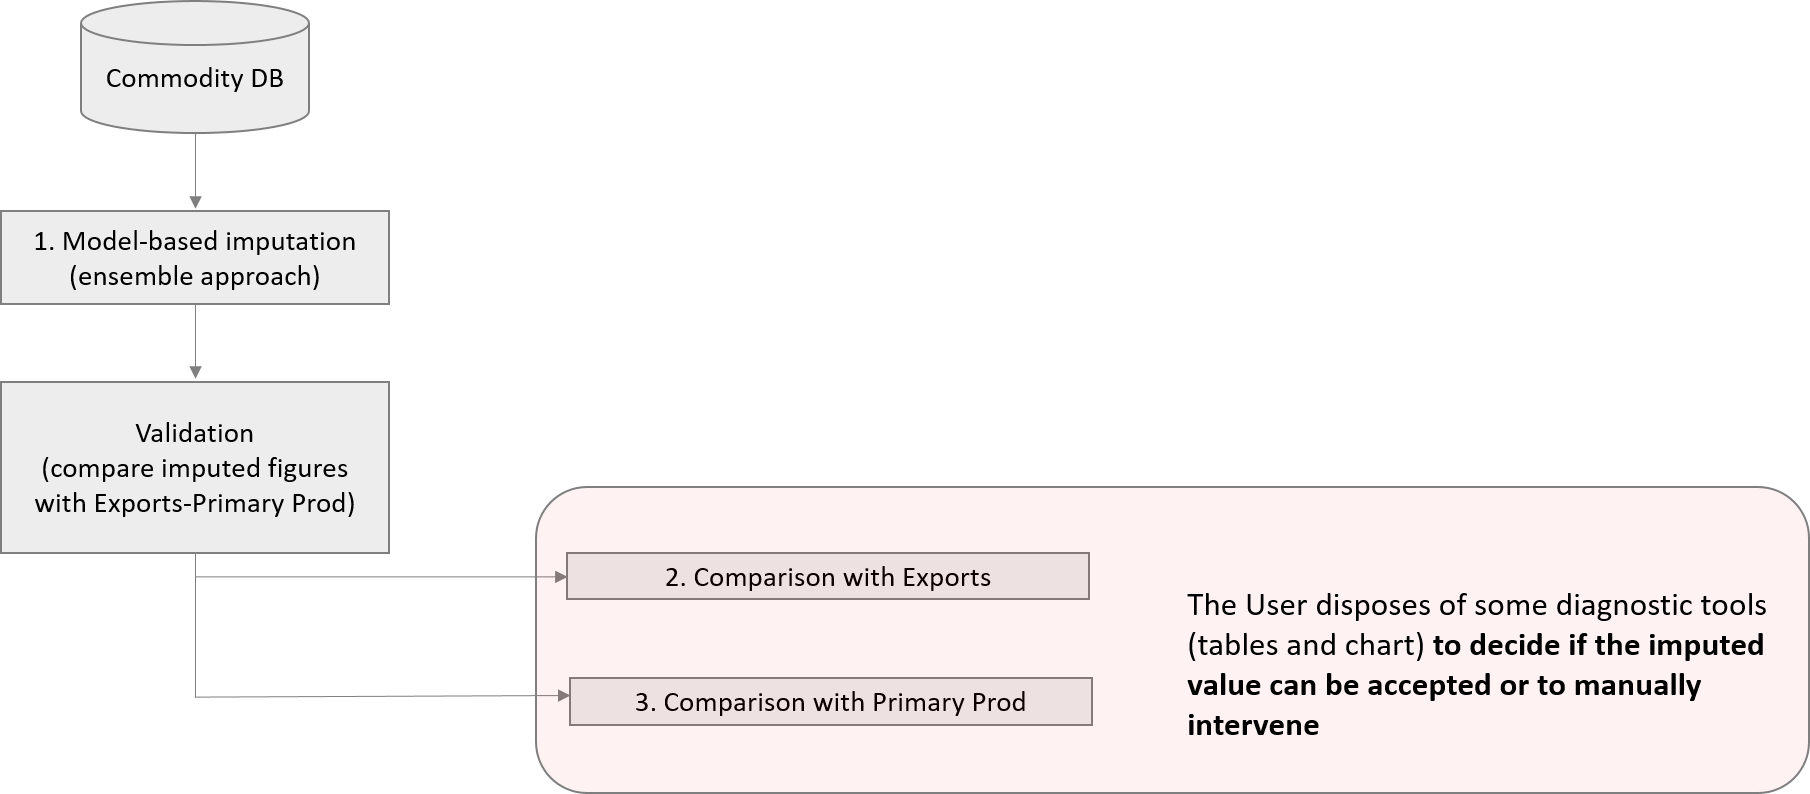
\includegraphics{plot/moduleWorkFlow.png}
\caption{Overall workflow}
\end{figure}

Being trade data the most realible, the first check performed consists in comparing imputed production data with Exports (and not to net trade as described in the ``Scenario 2'' paragraph.)

\begin{figure}
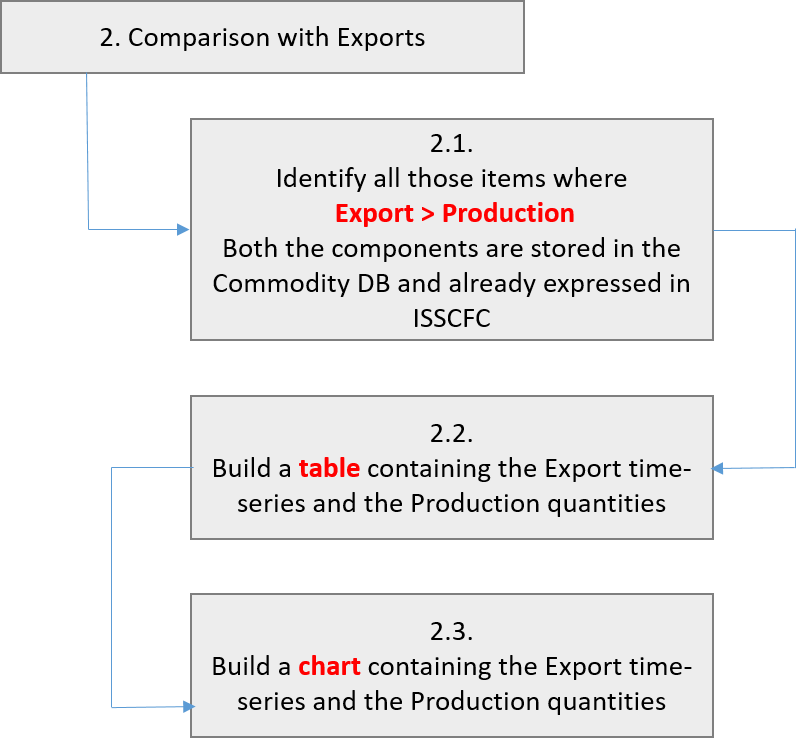
\includegraphics[height=6.5cm,width=5.85 cm]{plot/tradeCheck}
\caption{Trade check}
\end{figure}

The user will be supported by the application to visualize and validate all those items characterized by Exports higher than production. It has been explicitly requested that the comparison between the imputed production and export should include the complete export time-series\footnote{The idea is to give to the user the possibility to contextualize the production quantity within the complete export time-series.}.
At each run of the R plugin, the user who has launched the routine will be supported by a number of auxiliary tools:

\begin{itemize}
\item.csv table containing both production and export time-series (sent per email attachment);
\item  a set of .pfd files containing charts comparing production figures versus exports, only for those series where the exports exceed production at least for one year (sent per email attachment);
\item a simple Shine app where the user can interactively select the series to be displayed.
\end{itemize}

The same kind of tooling will be provided also to check if the primary availability is always
enough to produce the imputed ammount of processed goods.

Anyway, the comparison between derived and primary production is not as straightforward
as the one between processed production and exports. Due to the lack of a consolidated commodity-tree which could support the application in identifying those primary items that might have been used as input to produce the current processed good, a workaround has been developed to associate processed items to the corresponding primary products.

The idea is to use the ISSCAAP groups to associate all the processed and preserved items (in the commodity DB) expressed in terms of ISSCFC codes to the proper primary item(s). Given that each ISSCAAP group generally contains many primary items, the obtained matching will not be a one to one relation. This means that the check for the primary availability cannot be completely automated.



\begin{figure}
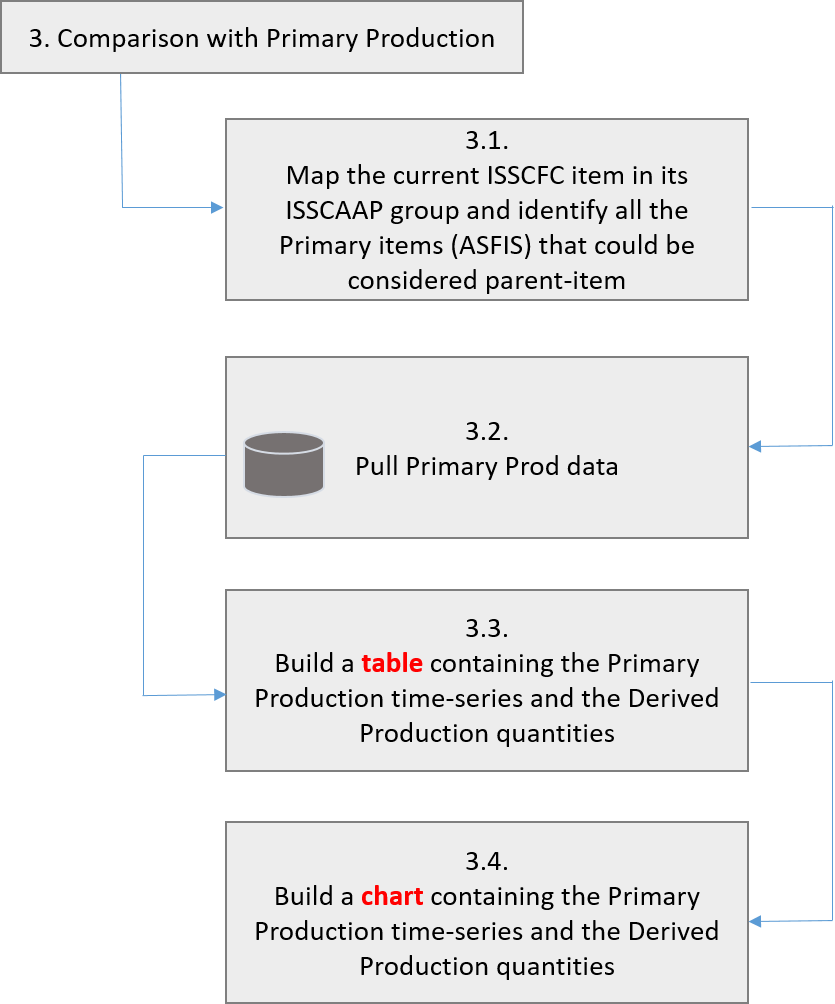
\includegraphics[height=7cm,width=4.84cm]{plot/PrimaryProdCheck.png}
\caption{Primary production check}
\end{figure}



\section{Classifications and data-set description}

The migration of the commodity DB in the SWS requests a number of preliminary operations:

\item Agree on the data-set structure, which columns\footnote{Columns of a datasets might also be referred as data-set dimensions.}, which classification\footnote{A classification (codelist) is associated to each dataset dimention (column). The codelist represent the columns domain: all the possible values the cell in the column can have. Any attempt to write in a cell a value/code that does not belong to the codelist previously associated to the column, will be rejected.}. Each numeric figure is uniquely  identified by the combination of four dimensions which are the primary keys of the data-set. For the commodity DB the primary keys are:

\begin{itemize}
\item { geographicAreaM49}
\item { measuredElement} 
\item { measuredItemISSCFC} - this classification does not exist yet in the SWS
\item { timePointYears} 
\end{itemize} 

Note that the name of the column/dimention usually matches with the name of the classification itself.
The following paragraph contains some observations about possible improvements to keep all the dataset dimensions the most standard as possible.

\paragraph{Country codes - } The current version of the commodity DB (stored in FishStatJ) already contains M49 codes for countries and ISSCFC for commodities. While the ISSCFC has not yet migrated, in the SWS there is a codelist called ``geographicAreaM49_fi''\footnote{geographicAreaM49_fi has been already used for the Primary Production dataset (Aquaculture and Capture).}. Apparently there is no difference between the codes contained in geographicAreaM49 and those in geographicAreaM49_fi. The strong plea is to use the same classification in all the domains and to replace the current dimension geographicAreaM49_fi (in the already existing dataset) with the geographicAreaM49 fully validated and compliant with UNSD country codes.


\paragraph{Element codes -} The Commodity DB contains mainly trade data plus the Production pf processed and preserved goods.
\begin{itemize}
\item Import (both quantities and values)
\item Export (both quantities and values)
\item Re-Export (quantities)
\item Production (quantities)
\end{itemize}


The following table contains a proposal to align FIAS elements codes to elements used in the Agriculture Production domain:

\begin{table}[h!]
  \begin{center}
    \caption{Element codes - mapping table}
    \label{tab:table1}
    \begin{tabular}{l|c|r} % <-- Alignments: 1st column left, 2nd middle and 3rd right, with vertical lines in between
      \textbf{Actual FIAS  code} & \textbf{Proposed code} & \textbf{Label} \\
      \hline
      61  & 5610 & Import quantity [tons]\\
      91  & 5910 & Export quantity [tons]\\
      62  & 5610 & Export value [\$]\\
      92  & 5910 & Import value [\$] \\
      221 & ---- & re-exporta quantity [tons]\\
      51 & 5510 & Production [tons] \\
    \end{tabular}
  \end{center}
\end{table}

\section{Module workflow}



\section{Annex 1 - Questionnaire Teplate - FC1 (see the proper attachement) }

\end{document}
